% !TeX root = ../Bachelorarbeit.tex
\chapter{Konzeption}
\section{Sichere Webseiten}
Einige wichtige Fakten zu Webseiten, die bei der Konzeption des Prototypen berücksichtigt werden müssen:

\begin{itemize}
\item \textbf{Immer mehr Nutzer sorgen für mehr Authentifikationen pro Sekunde und damit für eine höhere Auslastung}

Webseiten besitzen immer mehr und mehr Nutzer \cite{A31}. Mittlerweile besitzen über 50\% der Menschen weltweit einen Internetzugang und damit Zugriff auf die Vielfalt des World Wide Web \cite{A30}. Für Webseitenbetreiber bedeutet diese Entwicklung zunächst einmal das es sehr viel mehr potenzielle Aufrufe auf Webseiten pro Sekunde gibt. Daraus ergibt sich, dass es auf den verschiedenen Diensten auch mehr Authentifikationen pro Sekunde (im Vergleich zu vorher) gibt. Der Prototyp sollte in der Lage sein, Nutzer unabhängig voneinander zu bearbeiten ohne einen bestimmten Service zu blockieren. Dazu müssen von vorneherein begründet die richtigen Werkzeuge (und Programmiersprachen) verwendet werden, die dieses Vorhaben überhaupt erst möglich machen.

\item \textbf{Webseiten sind über das offene Netz zugänglich und bieten damit eine große Angriffsfläche für Brute-Force Angriffe}

Die berühmtesten Webdienste wie Netflix, YouTube und Facebook sind aus dem Internet erreichbar. Daher ist es nicht verwunderlich, dass gerade diese Webseiten Ziel von Bruteforce Angriffen werden können. Das gibt einem Angreifer die Möglichkeit, gezielt eine Liste von gebreachten Usernamen und Passwörtern auf verschiedenen Diensten durchzuprobieren. Meist sind diese Dienste in der Lage, die IP-Adresse des Angreifers zu blockieren falls zu viele Anfragen in einer gewissen Zeitspanne eingehen, dies umgehen die Angreifer dann allerdings mit Proxylisten und erzwungenen Wartezeiten vor jedem Angriff (z.B: nur 100 Accounts pro Proxy alle 60 Sekunden ausprobieren). Der Prototyp sollte Brute-Force Angriffe möglichst verhindern, indem vor der Webseite eine Firewall installiert wird, die die eingehenden Anfragen überprüft. Gehen vermehrt Anfragen aus einem bestimmten Land oder einem bestimmten IP-Bereich ein, muss dies erkannt und gebannt werden.

\item \textbf{Webseiten besitzen mehr Möglichkeiten als je zuvor um Nutzer zu authentifizieren, von dem muss sie aber erst Gebrauch machen}

Die alleinige Möglichkeit der Authentifikation durch verschiedene Faktoren genügt heutzutage nicht mehr aus. Wie beim Stand der Forschung zur adaptiven Multifaktorauthentifikation bereits erläutert, schreitet die Digitalisierung rasant voran. Dies zwingt Webseitenbetreiber dazu, die neuen Verfahren wie die TOTP - Authentifikation oder das WebAuthn auch zu unterstützen. Die besten Verfahren sind sonst unbrauchbar, wenn es keine Dienste gibt, die sie umsetzen. Aus dem folgt, dass der Prototyp verschiedene Authentifikationsmethoden anbieten muss, um der Digitalisierung des 21. Jahrhunderts gerecht zu werden. Neben dem Passwort sollte es mindestens ein (besser wären sogar 2 oder mehr) Verfahren geben, die sich an einem der zwei weiteren Kategorien des Besitzes und der Biometrie bedienen.

\item \textbf{Webanwendungen speichern üblicherweise Nutzerkonten bzw. personenbezogene Daten}

Der Datenschutz erfordert angemessene Vorsichtsmaßnahmen bei dem Umgang mit diesen Daten. So ist die Passwortdatei gegen unberechtigtes Kopieren zu sichern, Passwörtern müssen auf dem Rechner des Nutzers verschlüsselt und dann übertragen und fehlerhafte Anmeldeversuche protokolliert werden \cite{A32}.

Der Prototyp sollte vor allem Passwörter nicht im Klartext übertragen (falls unsichere Verbindung) und in keinem Falle im Klartext in Datenbanken persistieren. Sehr persönliche Daten wie zu Fingerabdrücken sollten möglichst gar nicht in Datenbanken persistiert werden. Dies müssen sie bei der Nutzung entsprechender Schnittstellen wie WebAuthn allerdings auch nicht um eine sichere Authentifikation zu gewährleisten.

\item \textbf{Webnutzer sind oft unvorsichtig mit Passwörtern und wählen zu leichte}

Wie bereits gezeigt, neigen Nutzer zu sehr einfachen Passwörtern. Daher müssen einfache Passwörter wie ``1234'' im Vorhinein bereits ausgeschlossen werden. Man könnte eine Liste mit häufig genutzten Passwörtern verwenden, die den Nutzer vor der Wahl eines zu einfachen Passwortes hindert. Am einfachsten ist es eine Passwort-Policy Strategie zu wählen, die eine Mindestlänge des Passwortes voraussetzt. Dies macht das Passwort bei missbräuchlicher Nutzung zwar auch nicht sehr viel sicherer, ist aber ein Schritt in die richtige Richtung.

\end{itemize}
\newpage

\section{Auswahl der Authentifizierungsverfahren}
Bei der Auswahl der Authentifizierungsverfahren musste vor allem berücksichtigt werden, inwiefern das Verfahren im Rahmen dieser Arbeit umsetzbar ist. Dies bezieht sich einerseits auf die Zeit, die es für die Implementation benötigt und andererseits auch auf die monetäre Machbarkeit. Es existieren für die Webauthentikation zum Beispiel ganz spezielle USB-Sticks von angesehenen Marken, die allerdings einige hunderte Euro kosten. Die Features die sie im Gegensatz zu einem ganz normalen USB-Stick (FIDO USB) liefern, beziehen sich dabei nur auf den Teil der Userverifikation. So besitzen einige USB-Sticks einen eingebauten Fingerabdrucksensor, ein Tastenfeld oder sogar zusätzliche Sicherheitssoftware auf den Massendatenträgern. Innerhalb dieser Arbeit sollte es allerdings um den Einsatz eines solchen Verfahrens für den Durchschnittsnutzer innerhalb von Unternehmen oder einen Casual Surfer gehen. Eine teure Anschaffung für die eigene Sicherheit erscheint dem Durchschnittsnutzer als nicht nötig.

Das Verfahren des Usernamen und des Passwortes wurde gewählt, weil es zum Verfassungszeitpunkt dieser Arbeit die Nutzer von Webseiten meist alleinig sichert. Die Loginverfahren größerer Dienste wie Microsoft Outlook, Google Mail und Facebook besitzen zwar schon seit Jahren die Möglichkeit der Authentifikation mit einem zweiten Faktor, doch das sind eher Ausnahmen. Ein Großteil der Internetpräsenzen ist sich entweder nicht der Risiken von Passwörtern für ihre Nutzer bewusst oder kann sich den Mehraufwand von neuen Verfahren nicht leisten. Gleichzeitig war es im Rahmen dieser Arbeit wichtig eine typische Implementation mit Username \& Passwort und ihren Scheinsicherheiten wie Hashes mit Salt und Pepper zu präsentieren. Es ist wichtig, den Ist-Zustand im heutigen Internet zu verstehen, um die Vorteile von neueren Methoden nachzuvollziehen.

Eine dieser neuen Methoden ist das zweite Verfahren. Nach dem Passwort ist das wohl der häufigste zweite Faktor den man findet. Apps wie der 'Google Authenticator' zählen mittlerweile als Synonym für das \ac{totp} - Verfahren wie es im RFC beschrieben ist. Dies liegt unteranderem auch daran, dass die App tatsächlich die recht strikten Vorgaben aus dem RFC befolgt und nur minimale Unterschiede dazu aufweist.
\newpage

An dieser Stelle stellte sich eher die Frage ob HOTP oder \ac{totp} in den Prototypen implementiert werden sollte. Es wurde sich für das \ac{totp} - Verfahren entschieden, da es zwar den Mehraufwand der Synchronisation zwischen Zeit des Gerätes und des Servers benötigt doch dafür die Sicherheit der begrenzten Zeit bietet wie bereits erläutert.

Das dritte Verfahren, die 'Web Authentication', ist wohl das Erforschungswürdigste der drei Verfahren. Sie ist von allen drei Verfahren am seltensten auf Internetseiten vertreten und da stellt sich nach einer Analyse des Mehrwertes dieses Verfahrens die Frage nach dem Grund dafür. Im Gegensatz zu den anderen beiden Authentifikationsmethoden wurde Dieses nicht für den Prototypen ausgewählt, weil es so weit verbreitet und bereits genutzt wird sondern genau im Gegenteil: Es wurde gewählt, um mögliche Gründe zu suchen weshalb das Verfahren der Webauthn heutzutage kein Standard darzustellen scheint. Es muss untersucht werden ob es starke Nachteile Gegenüber der anderen Verfahren bietet, denn im Ansatz scheint es alle Nachteile des Passwortes auszumerzen.
\newpage

\section{Authentifikation in drei Schichten}

\begin{center}
    \center
    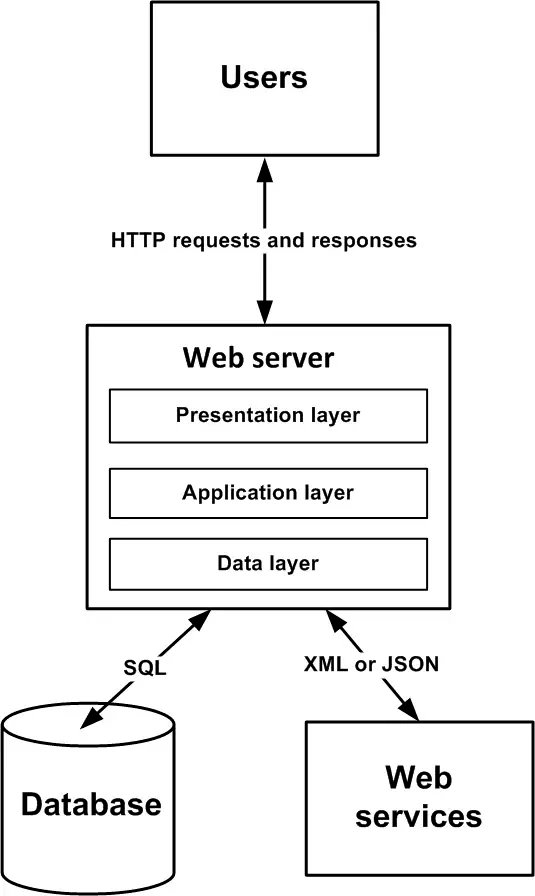
\includegraphics[width=10cm]{main-qimg-82af1fe49f85a31700d35570189a1fce.png}
\end{center} 

Das Ziel des Prototypen ist es, wie eingangs erwähnt, vorhandene Authentifizierungsverfahren abseits der klassischen UserID / Passwort Methode zu begutachten und dessen Schwächen aufzudecken. Daraus ergeben sich die typischen drei Komponenten von Drei-Tier-Client-Server Architekturen:

Ein Client, der Anfragen an die Applikation (das Backend bzw. den Server) sendet, welches die Daten dann in einer Datenbank mittels eines DBMS (Datenbankmanagementsystems) persistiert und verwaltet. Wie auch im Bild zur 3 Tier Architektur zu sehen, agiert der User auf dem Presentation Layer, stellt Anfragen bzw. sendet JSON Objekte an den Server, der die entsprechenden Webservices liefert. Der Server speichert keine States, wodurch der Nutzer typischerweise mit jeder Anfrage alle benötigten Informationen liefern muss. Der Server liefert demnach lediglich die \ac{rest} Schnittstellen. Implementationsdetails und weitere Informationen zum Prototypen gibt es in folgenden Kapiteln.

\section{Anforderungen and den Prototypen}
Auch wenn die Frage: ``Ist eine gelungene Authentifikation auch eine erfolgreiche Authentifikation?'' eine philosophische zu sein scheint, ist sie dennoch nicht minder interessant. Es wurde bereits gezeigt, dass Nutzer nicht gewillt sind komplizierte und aufwendige Dinge zu tun, um sich selbst und ihre Daten im Internet zu schützen. Sofern also die Methodik der Webseite zu kompliziert ist, sucht der Nutzer sich Ausflüchte um die vorhandenden Verfahren so angenehm wie möglich zu machen, was wiederrum die Sicherheit ihrer Internetpräsenz gefährdet. Das Passwort besitzt zu viele Schwachstellen als das man eine Authentifikation damit als Erfolg verbuchen kann. Es scheint eher dem Zweck 'irgendeiner Schutzbariere zwischen fremder Person und Daten des Nutzers' zu dienen als wirklich zur 'Sicherheit'.

\begin{itemize} 
\item \textbf{Nutzerfreundlichkeit}

Angefangen der Nutzerfreundlichkeit, einem der wichtigsten Kriterien für die Authentifikation, welches in direktem Bezug zur Sicherheit steht \cite{A24} \cite{A25} \cite{A26}. Der Prototyp soll eine einfache Authentifikation ermöglichen. Keine häufigen Weiterleitungen, keine Popups, keine langen Ladezeiten und vorallem zwecks Authentifizierung: Keine sinnfreie Aneinanderschaltung von verschiedenen Sicherheitsfaktoren.
\newpage

Ein Beispiel für solch eine Praktik wäre, dass nach der Bestätigung des Einloggvorgangs durch Fingerabdruck zusätzlich eine PIN und in folge dessen ein Sicherheitsschlüssel (mit zusätzlich benötigtem PIN) verlangt wird, obwohl nach dem ersten Schritt des Fingerabdrucks bereits die Authentizität des Users festgestellt wurde. So muss der Prototyp am Besten aus nur einem Faktor der Sicherheit bestehen und dem Nutzer die Auswahl zur Selbstentscheidung über die verschiedenen Möglichkeiten bieten, so wie es bei der adaptiven MFA (anhand von selektierten Faktoren) auch der Fall ist. Im konkreten Fall des Prototyps soll es demnach auch reichen nur einen der registrierten Geräte für die Web Authentication zu nutzen, so kann der User bequem die PIN zur Authentifizierung nutzen. Falls der Rechner dies nicht unterstützt, kann der User zum Sicherheitsschlüssel greifen oder das Smartphone für das \ac{totp} - Verfahren verwenden.

\item \textbf{Sicherheit}

Die Sicherheit einer Webanwendung hängt primär von ihrem Schutzbedarf ab. Viele Softwareentwickler setzen sich nur widerwillig mit dem Thema außeinander, oder in den vergangenen Jahren eher notgedrunken durch die Kunden. Dabei sind die Ursachen teilweise auch UX-Fehlern zuzuschreiben, weshalb der 'Secure by Design' Ansatz befolgt werden sollte \cite{A27}.

Der Prototyp sollte zur Sicherung der Kunden möglichst unnötige Metadaten vermeiden. Dazu sollen meist die selben Statuscodes und nur allgemeine Fehlermeldungen bei nicht erfolgreicher Authentifikation zurückgegeben werden. So ist die Nachricht ``Das Passwort ist inkorrekt.'' als obsoluter Fehler zu betrachten, da ein Angreifer nun die Möglichkeit hat, durch einen Bruteforce - Angriff auf das Loginformular das richtige Passwort zu erraten. Diese Nachricht würde nämlich implizieren, dass ein Nutzer mit eingegebenem Nutzernamen in der Datenbank vorhanden ist, doch das Passwort nicht stimmt. Stattdessen werden allgemeine Responsemessages gegeben wie ``Der Benutzername oder das Passwort sind falsch.'', um dem Angreifer keinerlei Metadaten auszuhändigen. Gleichzeitig muss die Verbindung zum Backend, auch im Prototyp, durch ein eigenes SSL - Zertifikat gesichert sein. \ac{mitm} - Angriffe sind, wie bereits erläutert, nicht immer verhinderbar. In unserem Falle sind wir selbst der Aussteller des Zertifikats und vertrauen uns selbst. Ein User kann (und wird) allerdings nicht die Vertrauenswürdigkeit seines Zertifikates erfragen.
\newpage

Wenn man die drei Verfahren nach ihrer Sicherheit ordnet, käme an hinterster Stelle wohl das Passwort. Wieso wurde bereits erläutert. Darauf würde das \ac{totp} - Verfahren kommen, das so lange sicher ist wie das Gerät welches die \ac{totp} - Codes erfragt sicher ist.

Hat man seinen QR-Code also im Google Authenticator eingescannt und lässt sein Smartphone ungesichert an einem öffentlichen Ort liegen, kann ein Angreifer sich das Smartphone nehmen, die App öffnen und den Code auf der Webseite eingeben. Das sicherste Verfahren (aus den ausgewählten im Rahmen dieser Arbeit) ist die Webauthentikation. Sie bietet wenig Angriffsfläche, dadurch das die privaten Schlüssel an einem sicheren Ort im Betriebssystem persistiert werden und es demnach in der Verantwortung des Betriebssystems liegt diese zu sichern. Der öffentliche Schlüssel besitzt keinen Wert und wird vom Authenticator generiert. Dadurch ist kein Zutuen des Nutzers erforderlich wie bei einem Passwort. Dieses Verfahren ist auch relativ sicher gegen \ac{mitm} - Angriffe, da ein Angreifer maximal die Challenge des Servers abfangen kann, um sein eigenes Gerät für einen Nutzer zu registrieren. Dies erfordert allerdings entweder eine komplette Kontrolle über den Rechner (Remote Access Control) oder phsysischen Zugriff auf den Rechner durch den Angreifer.

\item \textbf{Datenschutz}

Der Datenschutz ist ein Element der Sicherheit \cite{A28}, welches als ``Vertraulichkeit'' auch in den Grundwerten des IT-Grundschutzes wiederzufinden ist. Die Forschungsfrage dieser Arbeit ist überhaupt erst entstanden, durch einen Datenschutzvorfall bei Firmen. Auch wenn der Datenschutz bis jetzt nicht viel Erwähnung fand, ist er neben der Sicherheit und der Nutzerfreundlichkeit kein minderes Kriterium für eine erfolgreiche Authentifikation. Zum Schutz der Daten gehört zum Beispiel, SQL - Injektionen durch das Benutzen von 'Prepared SQL Statements' \cite{A28} zu verhindern. Dies bedeutet, dass Userdaten an keiner Stelle unformatiert in ein SQL Schnipsel eingebaut werden. Gleichzeitig muss sichergestellt werden, dass der Prototyp bei erfolgreichem Login keinerlei Metadaten über den Nutzer preisgibt. So wäre es ein Datenschutz-Problem wenn bei der Authentifikation über Webauthn zusätzliche Daten wie die E-Mail des Nutzers, sein Passwort und die Zeit der Erstellung des Accounts mitgesendet werden. Das Prinzip sollte stets lauten: So wenig Daten wie nötig. Das Recht auf informelle Selbstbestimmung \cite{A29} ist hier insofern gewährleistet, dass der User selbst entscheiden kann, ob er einen \ac{totp} registriert oder welches Gerät er für die Webauthn nimmt.
\newpage

Ein großer Vorteil neuerer Verfahren ist, dass hinter einer \ac{totp} oder Webauthn - Geräteregistration keinerlei persönliche Daten stehen. Selbst wenn Angreifer also den gesamten Registrationsprozess auf dem Gerät mitschneiden, können sie daraus keine verwertbaren Metadaten für zukünftige Angriffe erlangen.
\end{itemize}
